\speaker{\Mathieu}

\begin{frame}
\frametitle{M\underline{V}C : Les vues}
\begin{figure}[!h]
	\begin{center}
	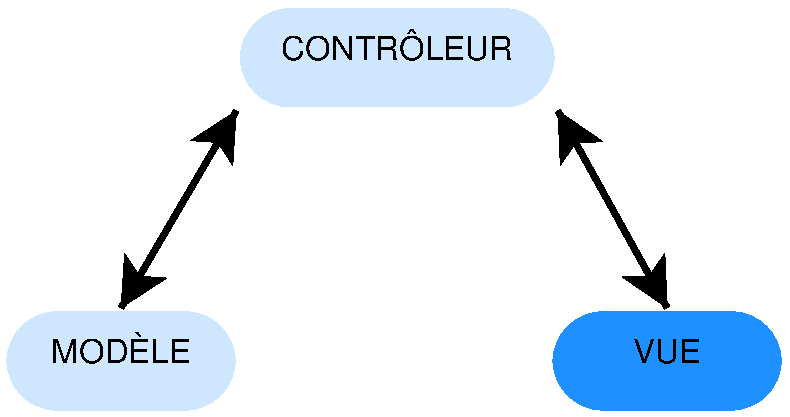
\includegraphics[scale=0.5]{images/mvcVue}
	\caption{Architecture M\underline{V}C}
	\end{center}
\end{figure}
Vue : partie visible, IHM(Interface Homme Machine)
\end{frame}

\begin{frame}
\frametitle{M\underline{V}C : Les vues}
\begin{block}{Vocabulaire}
\textbf{Template} : définit l'habillage d'une page, la position de ses éléments
\end{block}
\begin{figure}[!h]
	\begin{center}
	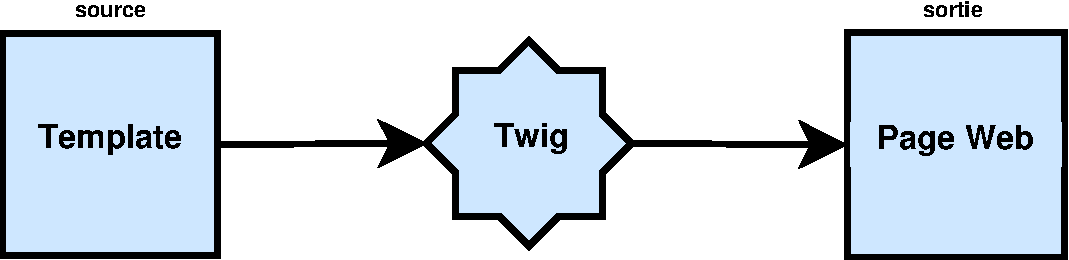
\includegraphics[scale=0.5]{images/twig}
	\caption{Fonctionnement du moteur de template Twig}
	\end{center}
\end{figure}
\end{frame}

\begin{frame}
\frametitle{M\underline{V}C : Les vues}
Architecture des templates :
\begin{itemize}
\item Niveau 1 : Architecture générale pour l'ensemble des pages
\item Niveau 2 : Architecture spécifique pour chaque groupe de pages similaires
\item Niveau 3 : Templates finaux pour chaque page Web de l'application
\end{itemize}
\begin{figure}[!h]
	\begin{center}
	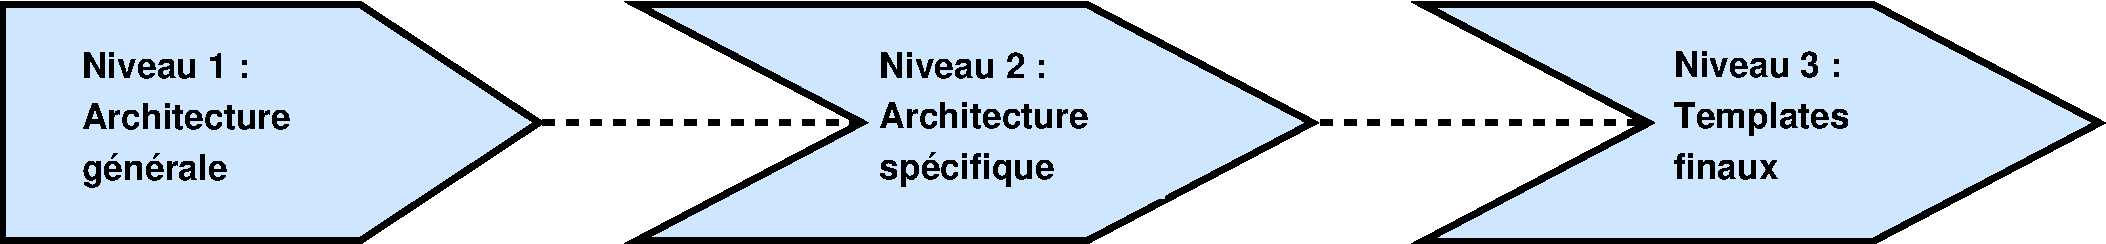
\includegraphics[scale=0.3]{images/archiTemplates}
	\caption{Imbrication des templates}
	\end{center}
\end{figure}
\end{frame}

\begin{frame}
\frametitle{M\underline{V}C : Les vues}
Utilisation d'une collection d'outils CSS : Bootstrap
\begin{itemize}
\item Gain de temps
\item Pris nativement en charge par Symfony
\item Permet d'avoir une application accessible depuis tout type d'appareil (ordinateur, tablette, smartphone)
\end{itemize}
\end{frame}

\begin{frame}
\frametitle{M\underline{V}C : Les vues}
\begin{figure}[!h]
	\begin{center}
	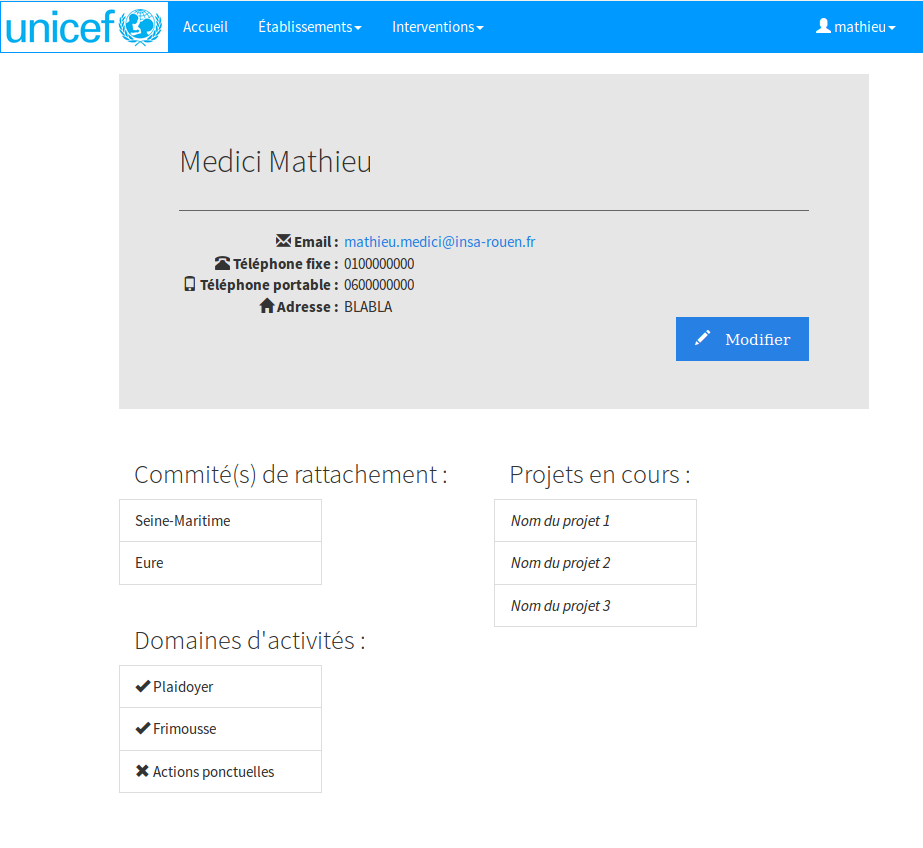
\includegraphics[scale=0.165]{images/profil.png}
	\caption{Page de profil d'un utilisateur}
	\end{center}
\end{figure}
\end{frame}

\begin{frame}
\frametitle{M\underline{V}C : Les vues}
Affichage d'une autre vue
\end{frame}